\documentclass{article}

% if you need to pass options to natbib, use, e.g.:
% \PassOptionsToPackage{numbers, compress}{natbib}
% before loading nips_2017
%
% to avoid loading the natbib package, add option nonatbib:
% \usepackage[nonatbib]{nips_2017}

\usepackage{nips_2017}

% to compile a camera-ready version, add the [final] option, e.g.:
% \usepackage[final]{nips_2017}

\usepackage[utf8]{inputenc} % allow utf-8 input
\usepackage[T1]{fontenc}    % use 8-bit T1 fonts
\usepackage{hyperref}       % hyperlinks
\usepackage{url}            % simple URL typesetting
\usepackage{booktabs}       % professional-quality tables
\usepackage{nicefrac}       % compact symbols for 1/2, etc.
\usepackage{microtype}      % microtypography

\usepackage{graphicx} % more modern
\usepackage{caption}
\usepackage{subcaption}
\usepackage{wrapfig}

% AMS stuff
\usepackage{amsmath, amsthm, amssymb}
\usepackage{dsfont}
\newtheorem{theorem}{Theorem}
\newtheorem{lemma}{Lemma}
\newtheorem{cor}{Corollary}

% For algorithms
\usepackage{algorithm}
\usepackage{algorithmic}

\usepackage{booktabs}
%\newcommand{\theHalgorithm}{\arabic{algorithm}}

\DeclareMathOperator*{\argmin}{arg\,min}
\DeclareMathOperator*{\argmax}{arg\,max}
\usepackage{xspace}
\newcommand*{\eg}{e.g.\@\xspace}
\newcommand*{\ie}{i.e.\@\xspace}

\usepackage{color}
\newcommand{\todo}[1]{{\bf \color{red}[todo: #1]}}

\title{Geometric Approach to Active Learning for CNNs}

% The \author macro works with any number of authors. There are two
% commands used to separate the names and addresses of multiple
% authors: \And and \AND.
%
% Using \And between authors leaves it to LaTeX to determine where to
% break the lines. Using \AND forces a line break at that point. So,
% if LaTeX puts 3 of 4 authors names on the first line, and the last
% on the second line, try using \AND instead of \And before the third
% author name.

\author{
  David S.~Hippocampus\thanks{Use footnote for providing further
    information about author (webpage, alternative
    address)---\emph{not} for acknowledging funding agencies.} \\
  Department of Computer Science\\
  Cranberry-Lemon University\\
  Pittsburgh, PA 15213 \\
  \texttt{hippo@cs.cranberry-lemon.edu} \\
  %% examples of more authors
  %% \And
  %% Coauthor \\
  %% Affiliation \\
  %% Address \\
  %% \texttt{email} \\
  %% \AND
  %% Coauthor \\
  %% Affiliation \\
  %% Address \\
  %% \texttt{email} \\
  %% \And
  %% Coauthor \\
  %% Affiliation \\
  %% Address \\
  %% \texttt{email} \\
  %% \And
  %% Coauthor \\
  %% Affiliation \\
  %% Address \\
  %% \texttt{email} \\
}

\begin{document}
% \nipsfinalcopy is no longer used

\maketitle

\begin{abstract}
Convolutional neural networks (CNNs) have been successfully applied to many recognition and learning tasks using a universal recipe; training a deep model on a very large dataset of supervised examples. However, this approach is rather restrictive in practice since collecting a large set of labelled images is very expensive. One way to ease this problem is coming up with smart ways for choosing images to be labelled from a very large collection (\ie active learning)

In this paper, we first show that existing active learning heuristics are not effective for CNNs even in an oracle case. Our counterintuitive empirical results make us question these heuristics and inspire us to come up with a simple but effective method, choosing a set of images to label such that they cover the set of unlabelled images as close as possible. We further present a theoretical justification for this geometric heuristic by presenting a bound over the generalization error of CNNs. Our experiments show that the proposed method significantly outperforms existing approaches in image classification experiments by a large margin.
\end{abstract}

\section{Introduction}
\todo{ saw just a couple of typos (lines 429, 641, 820).}
\todo{709: "have only access" ---> "only have access"

e.g. "The" is often missed from the start of "semi-supervised algorithm", e.g. on line 706, 782, 783

784 "having biased view" --> "having a biased view" 

785 "cause in inaccurate features"

e.g. on line 467 "since optimal solution" is missing "an/the"

542 "after each iteration of activate learning step" is missing "the"

Also, line 216 "our algorithm is agnostic to used semi-supervised" is in the wrong tense.}

Deep convolutional neural networks (CNNs) have shown unprecedented success in many areas of active research in computer vision and pattern recognition like image classification, object detection and scene segmentation. Although CNNs are universally successful in many tasks, they have a major drawback; they need very large amount of labelled data in order to be able to learn their millions of parameters. More importantly, it is almost always better to have more data since the accuracy of CNNs is often not saturated with increasing dataset size. Hence, there is a constant desire to collect more and more data. Although this behavior is rather desired from an algorithmic perspective (higher representative power is typically better), labelling a dataset is a time consuming and expensive task. These practical considerations bring a critical question: \emph{``what is the optimal way to choose data points to label such that the highest accuracy can be obtained given a fixed labeling budget.''} Active learning is one of the common paradigms to address this question.

The goal of active learning is to find effective ways to choose data points to label, from a pool of unlabelled data points, in order to maximize the accuracy. Although it is not possible to obtain a universally good active learning strategy \cite{dasgupta2004analysis}, there exist many heuristics~\cite{settles2010active} which have been proven to be effective in practice. To the best of our knowledge, almost none of these methods are utilized for deep learning since they typically are not effective for CNNs. The prevalent belief for this behavior is CNNs' tendency to make very confident mistakes. It is empirically observed that when CNNs make mistakes, they can assign arbitrary confidence values to their decisions. In other words, it is typically not possible to deduce that a CNN is uncertain and needs more data by solely looking at its outputs. Although we agree with this observation, our empirical analysis suggests that this is not the main reason behind the ineffectiveness of active learning for CNNs. 

Following our empirical study, we decide not to adopt an uncertainty based method and approach to the problem of active learning from a geometric perspective. We hypothesize that given a large unlabelled dataset, a desired property of the set of labelled points is to cover the set of unlabelled points as closely as possible \emph{(See Figure~\ref{fig:tsne} for a visual explanation)}. In other words, we find a set of points to label such that when they are labelled, every remaining unlabelled point in the dataset will have a close labelled neighbor. We formulate this space-covering property in terms of an optimization problem and present an efficient solution.

We carry out an in-depth analysis of our algorithm both theoretically and empirically. We study the generalization error of CNNs in a realistic setting and present a bound on the difference between the expected risk and the empirical risk of CNNs. We further consider the active learning case and present a bound over the risk of the unlabelled data points in terms of distance between unlabelled points and their labelled nearest neighbors. We further study the behavior of our proposed algorithm empirically for the problem of image classification using the CIFAR\cite{cifar} dataset. Our empirical analysis demonstrates state-of-the-art performance by a large margin. 

%In summary, contributions of this work are; i) first successful application of active learning on CNNs which is effective both with semi-supervision and without it, ii) an empirical study on limitations of uncertainty based active learning in CNNs, iii) theoreti 

\section{Related Work}
We discuss the related work in the following categories separately. Briefly, our work is different from existing approaches since $i)$ it specifically targets CNNs, $ii)$ our algorithm is effective with and without semi-supervision, and $iii)$ we theoretically analyze our algorithm.

\noindent\textbf{Active Learning}
Active learning has been widely studied and most of the early work can be found in the classical survey \cite{settles2010active}. It discusses most query strategies such as information theoretical methods \cite{mackay1992information}, ensemble approaches \cite{mccallumzy1998employing, freund1997selective} and uncertainty based methods \cite{tong2001support,lewissequential,joshi2009multi,li2013adaptive}. %We will try to review the literature coming after \cite{settles2010active}. 

Bayesian active learning methods typically use a non-parametric model like Gaussian process to estimate the expected improvement by each query \cite{kapoor2007active} or expected error after the queries \cite{roy2001toward}. These approaches are typically not applicable to deep learning scenarios since they do not scale to large-scale datasets. Ensemble methods are also not applicable to deep learning due to the large parameter space of neural networks. Such ensemble methods require an intractable number of networks to be trained to be effective.

One important class is that of uncertainty based methods, which try to find hard examples using heuristics like highest entropy \cite{joshi2009multi}, and geometric distance to decision boundaries \cite{tong2001support,brinker2003incorporating}. We present an empirical result in Section~\ref{sec:whatif} which motivated us to move away from such techniques. We empirically demonstrate that even in the oracle case, such algorithms are typically not effective for CNNs.

There are recent optimization based approaches which can trade-off uncertainty and diversity in order to obtain a diverse set of hard examples. Elhamifar~et al.  \cite{elhamifar2013convex} design a discrete optimization problem for this purpose and use its convex surrogate. However, the algorithm uses $n^2$ variables where $n$ is the number of data points. Hence, it does not scale to the deep learning case. There are also many discrete optimization based active learning algorithms designed for the specific class of machine learning algorithms like k-nearest neighbors and naive Bayes \cite{wei2015submodularity}. Even in the algorithm agnostic case, one can design a set-cover algorithm to efficiently cover the hypothesis space using sub-modularity \cite{guillory2010interactive, golovin2011adaptive}. Our algorithm can be considered to be in this class; however, we do not use any uncertainty information. Our algorithm is also the first one which is applied to CNNs.

Recently, a discrete optimization based algorithm \cite{BerlindU15} which is similar to ours has been presented for k-nearest neighbors type of algorithms in domain shift setting. Although our theoretical analysis borrows many techniques from \cite{BerlindU15}, their results are only valid for k-NN and are not applicable to CNNs. 

To the best-of-our-knowledge, the only active learning algorithm designed for CNNs is presented in \cite{wang2016cost}. It is a heuristic based transductive algorithm which assigns labels to data-points having high-confidence directly and queries labels for the ones having low confidence. We discuss its limitations in Section~\ref{sec:exp}.


\noindent\textbf{Unsupervised Subset Selection}
The closest literature to our work is the problem of unsupervised subset selection. This problem considers a fully labelled dataset and tries to choose a subset of it such that the model trained on the selected subset will perform as closely as possible to the model trained on the entire dataset. For specific learning algorithms, there are methods like core-sets for SVM \cite{tsang2005core} and core-sets for k-Means and k-Medians \cite{har2005smaller}. %However, there is no such method for CNNs.

The most similar to our algorithm is unsupervised subset selection described in \cite{wei2013using}. It uses a facility location problem in order to find a diverse subset covering the dataset. Our algorithmic difference is using a slightly different formulation of facility location problem. Instead of the min-sum, we use the minimax \cite{facility} form of the facility location. More importantly, we apply this algorithm for the first time to the problem of active learning and analyze our algorithm both empirically and theoretically.

 
\noindent\textbf{Semi-Supervised Deep Learning}
Our paper is also related to semi-supervised deep learning since we experiment the active learning both in fully-supervised and semi-supervised scheme. 
One of the early semi-supervised convolutional neural network algorithms was Ladder networks \cite{ladder}. Recently, we have seen adversarial methods which can learn a data distribution as a result of a two-player non-cooperative game \cite{salimans2016improved,gan_original,dcgan}. These methods are further extended to feature learning \cite{ali, bigan}. Thanks to the defined two-player game, these methods can perform semi-supervised learning naturally. We use Ladder networks in our experiments since adversarial architectures are notoriously hard to train. Our algorithm is agnostic to used semi-supervised learning algorithm and can readily be used in any semi-supervised or fully-supervised setting.

\section{Problem Definition}
\todo{By with/without semi-supervised, we meant 'semi-supervised' and 'fully-supervised', respectively. At each iteration, an active learning algorithm has two stages: 1. identifying a set of data-points and presenting them to an oracle to be labelled, and 2. training a classifier using these new as well as the previously labeled data-points. The second stage (training the classifier) can be done in a fully or semi-supervised manner. 'Fully-supervised' (i.e. without semi-supervision) is the case where training the classifier is done using only the labeled data-points. 'Semi-supervised' is the case where training also utilizes the points which are NOT labelled yet. We considered both cases and experimented on both. We will update the paper with a clarification on this terminology and include additional details in the camera ready.}

In this section, we formally define the problem of active learning and setup the notation for the rest of the paper. We are interested in a $C$ class classification problem defined over a compact space $\mathcal{X}$ and a label space  $\mathcal{Y}=\{1,\ldots,C\}$. We also consider a loss function $l(\cdot,\cdot;\mathbf{w}):\mathcal{X}\times \mathcal{Y} \rightarrow \mathcal{R}$ parametrized over the hypothesis class ($\mathbf{w}$), e.g.\ parameters of the deep learning algorithm. We also assume class-specific regression functions $\eta_c(\mathbf{x})=p(y=c|\mathbf{x})$ to be \mbox{$\lambda^\eta$-Lipschitz} continuous for each $c$.

We consider a large collection of data points which are sampled $i.i.d.$ over the space  $\mathcal{Z}=\mathcal{X}\times\mathcal{Y}$ as \mbox{$\{\mathbf{x}_i,y_i\}_{i \in [n]} \sim p_\mathcal{Z}$} where $[n]=\{1,\ldots,n\}$. We further consider an initial pool of data-points chosen uniformly at random among them as \mbox{$\mathbf{s}^0=\{s^0(j) \in [n]\}_{j \in [m]}$}.

An active learning algorithm has only access to $\{\mathbf{x}_i\}_{i \in [n]}$ and $\{y_{s(j)}\}_{j \in [m] }$. In other words, it can only see the labels of the points in the initial sub-sampled pool. It is also given a budget $b$ of queries to ask to an oracle and a (semi)supervised learning algorithm $A_{\mathbf{s}}$ which outputs a set of parameters $\mathbf{w}$ given a labelled set $\mathbf{s}$. The active learning with a pool problem can simply be defined as
\begin{equation}
\min_{\mathbf{s}^1 : |\mathbf{s}^1| \leq b} E_{\mathbf{x},y \sim p_\mathcal{Z}} [l(\mathbf{x},y; A_{\mathbf{s}^0 \cup \mathbf{s}^1})]
\end{equation}
In other words, an active learning algorithm can choose $b$ extra points and get them labelled by an oracle to minimize the future expected loss.

There are a few differences between our formulation and the classical definition of active learning. Classical methods consider the case in which the budget is 1 ($b=1$) but a single point has negligible effect in a deep learning regime hence we consider the batch case. It is also very common to consider multiple rounds of this game as in each round $k$, solving the following
\begin{equation}
\min_{\mathbf{s}^{k+1} : |\mathbf{s}^{k+1}| \leq b} E_{\mathbf{x},y \sim p_\mathcal{Z}} [l(\mathbf{x},y;A_{\mathbf{s}^{0} \cup \ldots  \mathbf{s}^{k+1} \cup \ldots  \mathbf{s}^{k+hor}})]
\end{equation}
Where $hor$ is the number of active learning iterations expected to be performed. Although it is more realistic, analysis is typically trickier in such a setting. Hence, we consider the myopic version and solve the single round of labelling as;
\begin{equation}
\min_{\mathbf{s}^{k+1} : |\mathbf{s}^{k+1}| \leq b} E_{\mathbf{x},y \sim p_\mathcal{Z}} [l(\mathbf{x},y;A_{\mathbf{s}^{0} \cup \ldots  \mathbf{s}^{k+1}})]
\end{equation}
In other words, our method solves the multi-stage problem in a myopic way without utilizing look-ahead. In the rest of the paper we discuss the fist iteration where $k=0$ for brevity although we apply it iteratively. We also consider a semi-supervised algorithm instead of a supervised one. Although, the query methods are typically equally applicable in both cases, we empirically observed different behavior. 

\section{Active Learning as a Set Cover}
In the non-Bayesian setting, the active learning problem is typically considered as refining decision boundaries by querying hard examples. Hence, using uncertainty is an empirically proven heuristic. However, this heuristic has very limited success in CNNs. This is widely attributed to the fact that the CNNs typically make very confident mistakes and the confidence values computed via soft-max outputs do not correspond to the true confidence of the CNN. Here, we focus on the following a rather more fundamental question; \emph{would classical query methods work for CNNs if CNNs had an accurate uncertainty estimate?}. Although the common sense answer is affirmative, our empirical analysis shows that this is typically not the case. We describe this experiment in detail in Section~\ref{sec:whatif}.

Empirical observation on ineffectiveness of uncertainty based approaches inspired us to design a rather non-intuitive method for active learning for CNNs. We propose to not use class estimates and/or labels of already labelled data points, but we instead attack the problem from a purely geometric perspective. We design an algorithm based on the heuristic of covering the set of unlabelled data points as closely as possible. We explain this algorithm in detail in Section~\ref{sec:alg} and further analyze it empirically in Section~\ref{sec:exp} and theoretically in Section~\ref{sec:analysis}.

\subsection{Ineffectiveness of Uncertainty based Methods}



\begin{wrapfigure}{t}{0.5\textwidth}
\vspace{-10mm}
  \begin{center}
    \begin{subfigure}[b]{0.23\textwidth}
		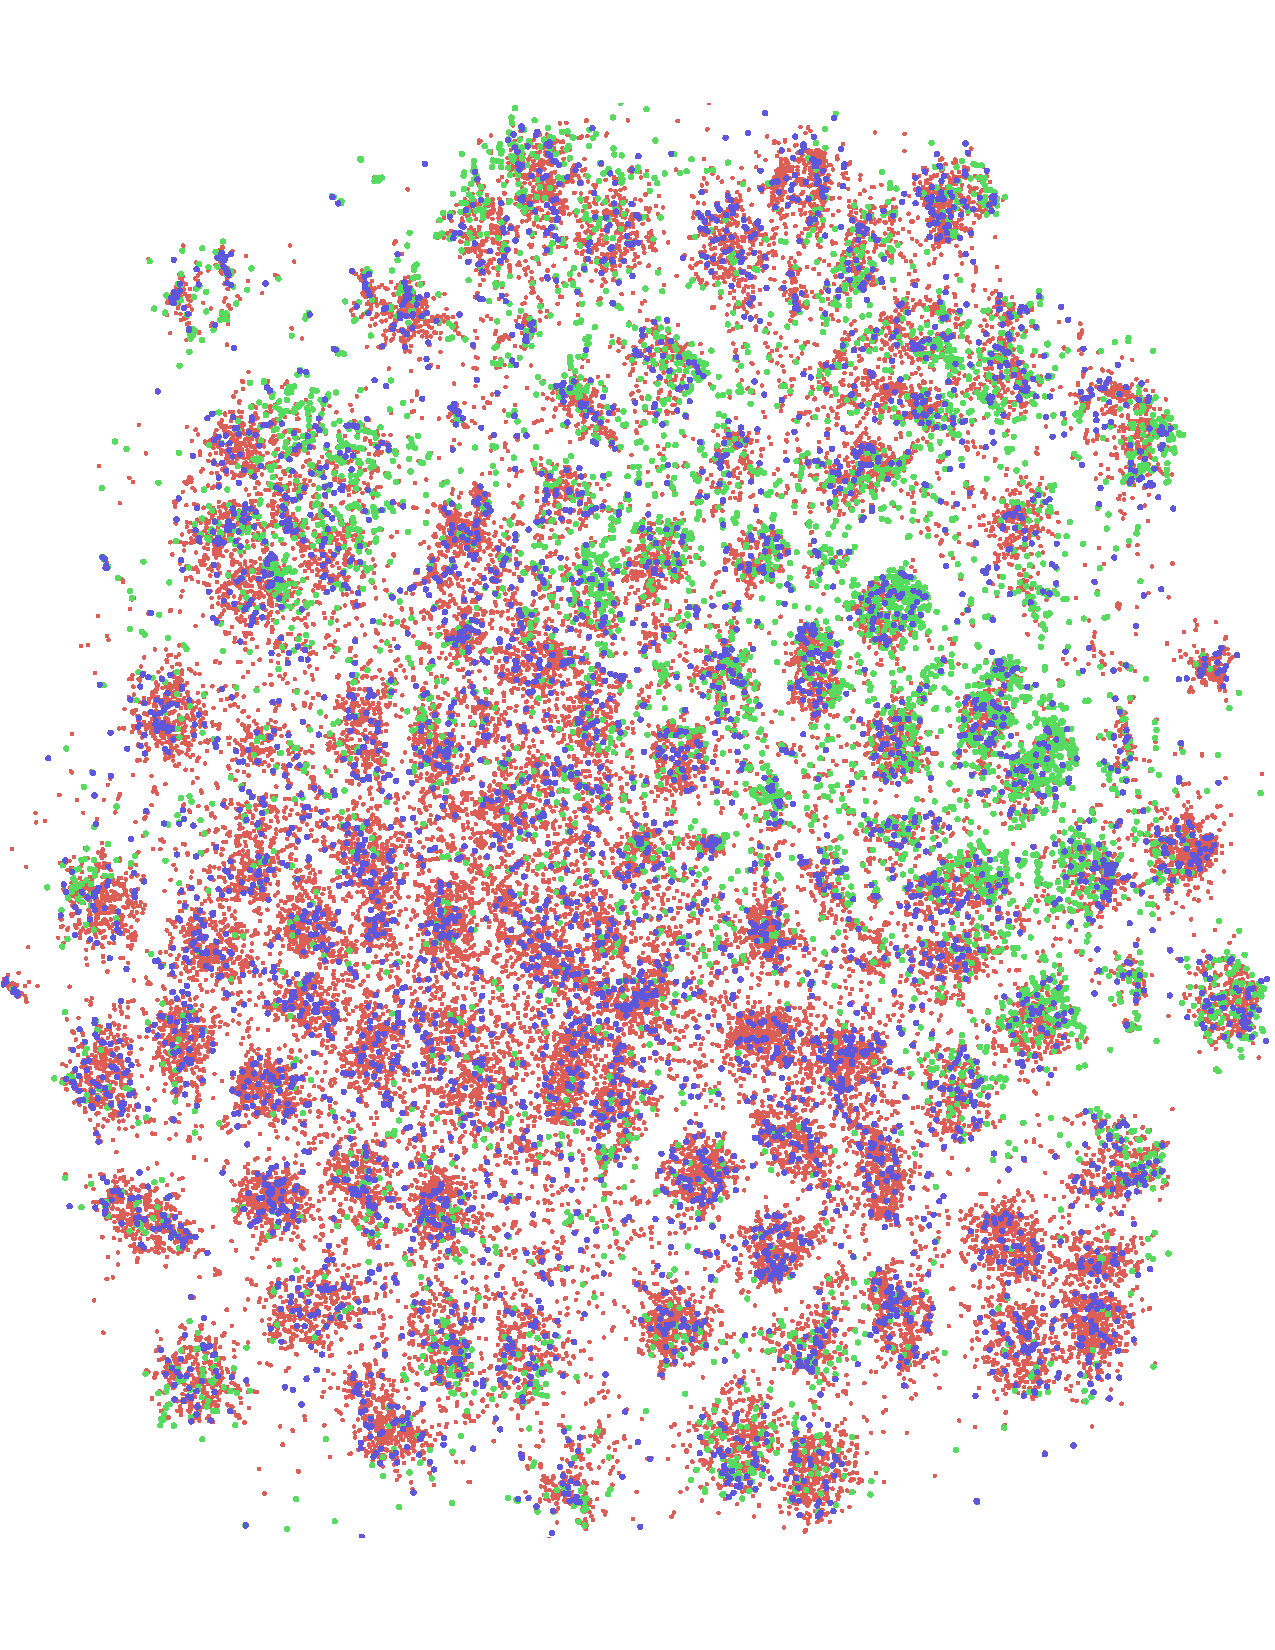
\includegraphics[width=\columnwidth]{fig1_a_1.pdf}
		\caption{Uncertainty Oracle}
    \end{subfigure}
    \begin{subfigure}[b]{0.23\textwidth}
		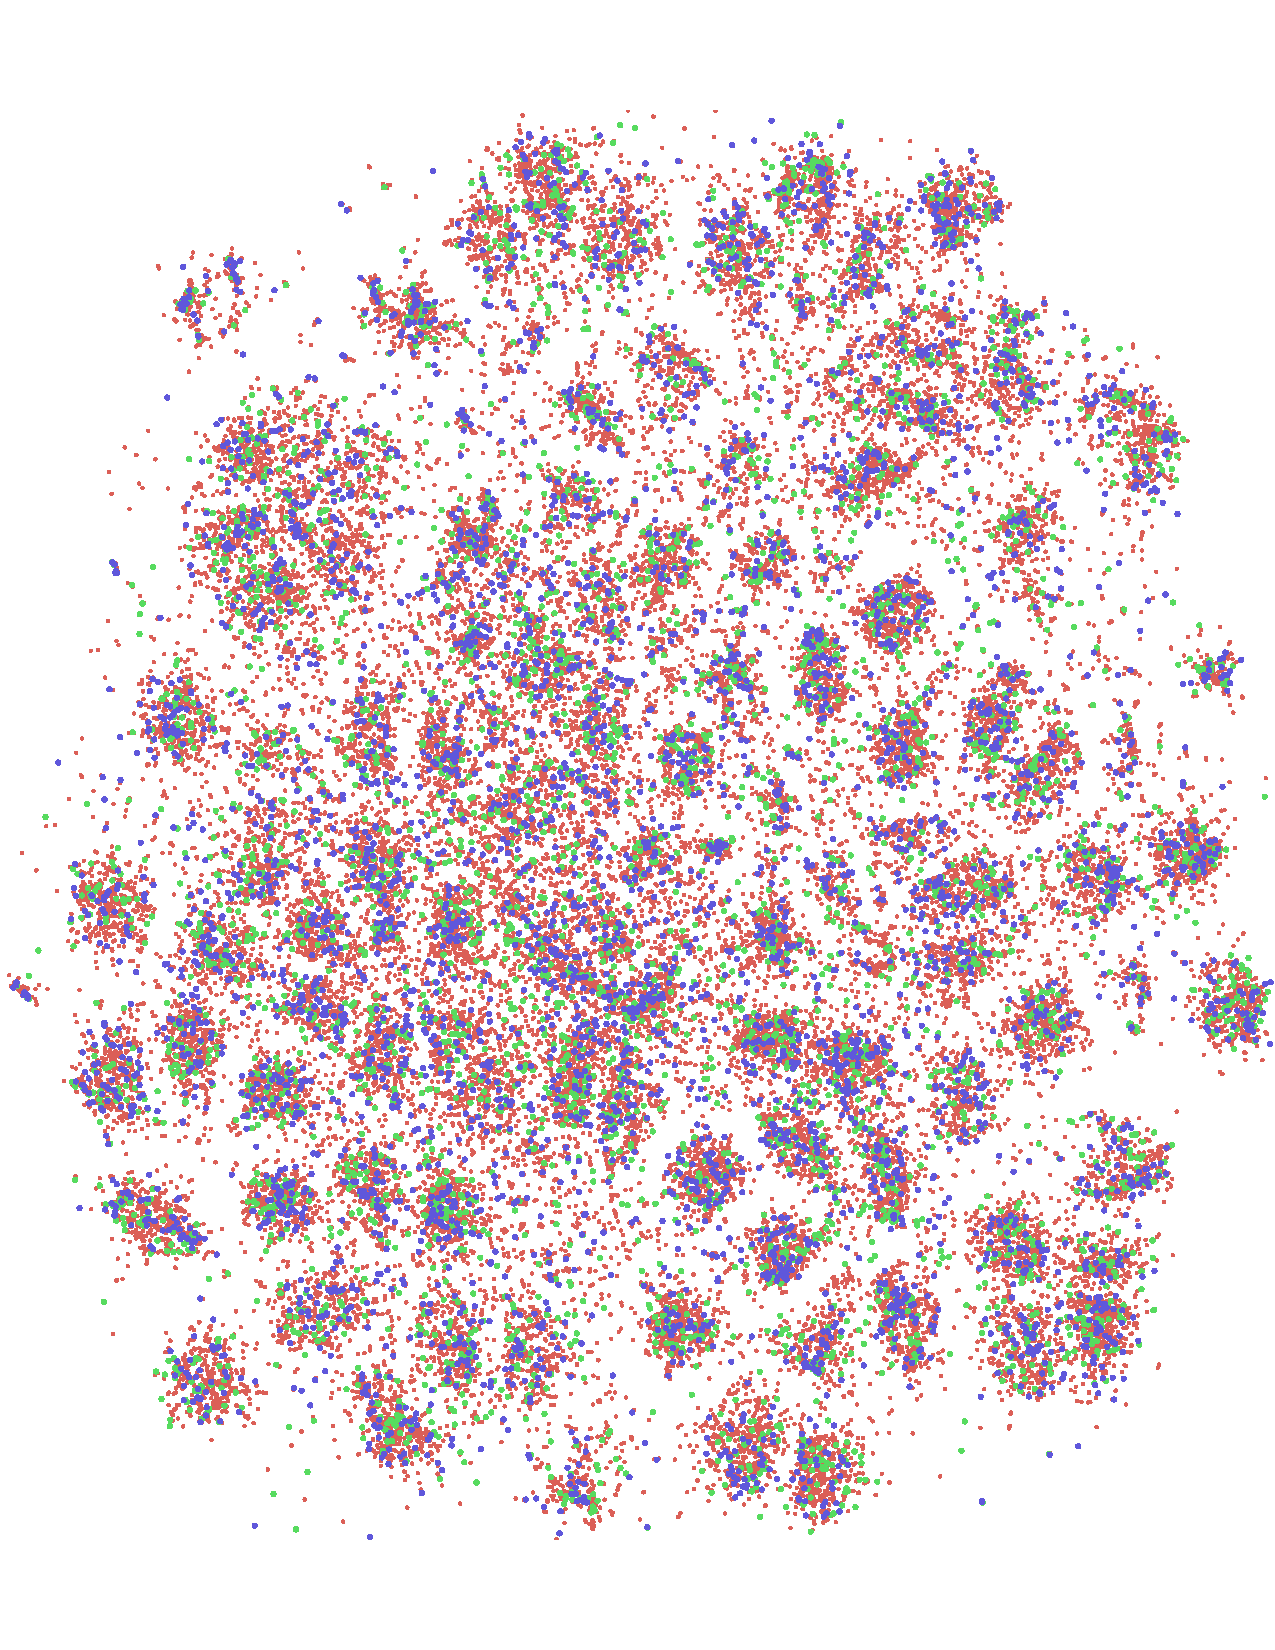
\includegraphics[width=\columnwidth]{fig1_b_1.pdf}
		\caption{Our Method}
    \end{subfigure}
\end{center}
{\small
    \caption{tSNE embeddings of images for active learning using uncertainty oracle and our algorithm. We further choose a step in active learning with 5000 images in initial pool ($|\mathbf{s}^0|=0$) and algorithms need to choose 1000 more samples $|\mathbf{s}^1|=5000$ and color the initial pool of images ($\mathbf{s}^0$) with blue, the actively chosen images ($\mathbf{s}^1$) with green, and remaining images ($[n] \setminus (\mathbf{s}^0\cup \mathbf{s}^1)$) with red. We can conclude from these visualizations that uncertainty oracle creates a bias leaving a significant part of the dataset uncovered. }}
\label{sec:whatif}
\vspace{-5mm}
\end{wrapfigure}


It is very common to attribute the ineffectiveness of uncertainty methods in CNNs to the fact that uncertainty estimates based on soft-max outputs are typically not accurate. Hence, it is very common to hypothesize the following:

\noindent\textbf{Hypothesis:} \emph{Deep learning algorithms lead to an inaccurate estimate of uncertainty hence the uncertainty based active learning methods fail with CNNs.}

Although this hypothesis is very intuitive considering the many confident mistakes CNNs typically make, it is also very easy to experiment with the following question;

\noindent\textbf{Question:} \emph{If CNNs produced accurate estimates of uncertainty, would uncertainty based active learning methods work for CNNs?}

We can answer this question by simply replacing the uncertainty estimate in active learning with oracle ground truth loss. In other words, we replace the uncertainty with $l(\mathbf{x}_i,y_i,A_{\mathbf{s}^0})$ for all unlabelled examples $\mathbf{x}_i$. Since this is the oracle for the estimation of the uncertainty, in practice the uncertainty based methods are expected to be upper bounded by this oracle. We sample the queries from the normalized form of this function by setting the probability of choosing the $i^{th}$ point to be queried as $p_i=\frac{l(\mathbf{x}_i,y_i,A_{\mathbf{s}^0})}{\sum_j l(\mathbf{x}_j,y_j,A_{\mathbf{s}^0})}$. We use two loss functions, classification accuracy \mbox{$\mathds{1}[y_i = \argmax_c CNN_c(\mathbf{x}_i;A_{\mathbf{s}^0})]$} and cross entropy
\mbox{$ - CNN_{y_i}(\mathbf{x}_i;A_{\mathbf{s}^0}) -\sum_{c \in [C] \setminus y_i} \log(1-  CNN_{c}(\mathbf{x}_i;A_{\mathbf{s}^0}))$} where $\mathds{1}[\cdot]$ is the indicator function and $CNN_c(\cdot,\mathbf{w})$ is the activation of $c^{th}$ softmax output given network weights $\mathbf{w}$. As the oracle, we use the maximum accuracy obtained by querying based on either of these loss functions. We perform this experiment with and without semi-supervision and plot the results in Figure~\ref{fig:neg}. \emph{(See Section~\ref{sec:imp} for implementation details)}

Results in Figure~\ref{fig:neg} suggest that even in the oracle case, uncertainty based methods are not effective for CNNs when compared with random sampling. We even observe that it causes the accuracy to drop in the semi-supervised case. Hence, the aforementioned hypothesis is not entirely correct and we can further conclude the following:

\noindent\textbf{Conclusion:} \emph{Inaccurate estimate of uncertainty does not explain the failure of uncertainty based active learning methods in CNNs. Active learning for CNNs requires rethinking.}

\todo{R1: I like the consideration of uncertainty-based methods to motivate your coverage-based approach. However, I do have a concern with the analysis Section 4.1. ... In practice it might be infeasible to update the parameters frequently after every single datapoint (mentioned in line 397), but an intermediate batch (<< 5000 points) size might yield a fairer analysis of uncertainty sampling.

In our experiments, we tried with batch size of 1k and observed the same behavior as in 5k (random sampling performed better than oracle uncertainty based method). On the other hand, we agree with the reviewer in the likely effect of correlation caused by the batch size. We will add a longer discussion and results for different batch sizes in the final version.}

We further discuss the failure of the uncertainty based oracle and try to motivate our method. Consider an embedding of images computed using the tSNE\cite{tsne} algorithm based on features learned after incorporating the entire dataset in learning. We plot the images in the initial pool ($\mathbf{s}^0$), chosen images for labelling ($\mathbf{s}^1$), and remaining images ($[n] \setminus (\mathbf{s}^0 \cup \mathbf{s}^1$)) with separate colors in Figure~\ref{fig:tsne}-a. As shown in Figure~\ref{fig:tsne}-a, the oracle algorithm samples the data points with a bias hence the resulting samples do not cover the space efficiently. A successful set of queries not only need to be hard but also need to cover the space. Hence, we believe covering the space effectively is very important for CNNs and we design an algorithm purely based on space covering in Section~\ref{sec:alg}. We also show the tSNE plot for our algorithm in Figure~\ref{fig:tsne}-b.

We believe this counterintuitive result is mostly due to the fact that we are sampling/labelling images in batches instead of querying one by one. Querying images one by one is not desired since a single point has no significant effect in deep learning due to the SGD. 

\begin{figure}[t]
\vspace{-3mm}
\includegraphics[width=\columnwidth]{fig1_2_h.pdf}
\vspace{-5mm}
\caption{Comparison of random sampling and active learning with oracle loss information. This figure suggests that even with oracle loss estimates, uncertainty based active learning algorithms are not effective for CNNs. Specifically for the case of semi-supervised learning, random sampling even outperforms oracle loss estimates. This is not surprising since semi-supervised algorithms relies heavily on feature learning and having a bias over the dataset would cause inaccurate feature learning.}
\label{fig:neg}
\end{figure}

\subsection{The Algorithm}
\label{sec:alg}
  \begin{wrapfigure}{R}{0.5\textwidth}
    \begin{minipage}{0.5\textwidth}
    \vspace{-8mm}
\begin{algorithm}[H]
   \caption{k-Center-Greedy}
      \label{alg:greedy}
\begin{algorithmic}
   \STATE {\bfseries Input:} data $\mathbf{x}_i$, existing pool $\mathbf{s}^0$ and a budget $b$
    \STATE Initialize $\mathbf{s}=\mathbf{s}^0$
   \REPEAT
   \STATE $u=\arg\max_{i \in [n] \setminus \mathbf{s}} \min_{j \in \mathbf{s}} \Delta(\mathbf{x}_i, \mathbf{x}_j)$
   \STATE $\mathbf{s} = \mathbf{s} \cup \{u\}$
   \UNTIL {$|\mathbf{s}|<b+|\mathbf{s}^0|$}
   \STATE {\bfseries return} $\mathbf{s} \setminus \mathbf{s}^0$
\end{algorithmic}
\end{algorithm}
\vspace{-8mm}
    \end{minipage}
  \end{wrapfigure}

We hypothesize that a good way to choose points to be labelled is trying to cover the unlabelled data points as close as possible. For example, consider a set of balls with radius $\delta$ centered at labelled points covering the entire unlabelled dataset. Intuitively, smaller $\delta$ should indicates a better the performance. Hence, we try to choose a subset of points which can minimize $\delta$ as an active learning strategy. 
  
    \begin{wrapfigure}{R}{0.5\textwidth}
    \begin{minipage}{0.5\textwidth}
    \vspace{-8mm}
\begin{algorithm}[H]
   \caption{Robust k-Center}
   \label{alg:bin}
\begin{algorithmic}
   \STATE {\bfseries Input:} data $\mathbf{x}_i$, existing pool $\mathbf{s}^0$, budget $b$ and outlier bound $\Xi$
   \STATE {\bfseries Initialize} $\mathbf{s}_g =$ k-Center-Greedy($\mathbf{x}_i, \mathbf{s}^0, b$)
   \STATE $\delta_{2-OPT} = \max_j \min_{i \in \mathbf{s}_g} \Delta(\mathbf{x}_i,\mathbf{x}_j)$ 
   \STATE $lb=\frac{\delta_{2-OPT}}{2}$, $ub=\delta_{2-OPT}$
   \REPEAT
   \IF {$Feasible(b, \mathbf{s}^0,\frac{lb+ub}{2},\Xi)$}
   \STATE $ub=\max_{i,j \mid  \Delta(\mathbf{x}_i,\mathbf{x}_j) \leq \frac{lb+ub}{2}}  \Delta(\mathbf{x}_i,\mathbf{x}_j) $
   \ELSE
   \STATE $lb=\min_{i,j \mid   \Delta(\mathbf{x}_i,\mathbf{x}_j) \geq \frac{lb+ub}{2}}  \Delta(\mathbf{x}_i,\mathbf{x}_j) $
    \ENDIF
   \UNTIL{$ub = lb$}
      \STATE {\bfseries return} $\{i\ s.t.\ u_i=1\}$
\end{algorithmic}
\end{algorithm}
\vspace{-5mm}
    \end{minipage}
  \end{wrapfigure}

Our algorithm is simply based on the \emph{k-Center} problem (minimax facility location problem \cite{facility}) which can intuitively be defined as follows; choose $k$ center points such that the largest distance between a data point and its nearest center is minimized. Formally, we are trying to solve:
\begin{equation}
\min_{\mathbf{s}^1} \max_i \min_{j \in \mathbf{s}^1 \cup \mathbf{s}^0} \Delta(\mathbf{x}_i,\mathbf{x}_j)
\end{equation}



Unfortunately this problem is NP-Hard \cite{cook}. However, it is possible to obtain a $2-OPT$ solution efficiently using a greedy approach shown in  Algorithm~\ref{alg:greedy}. If $OPT=\min_{\mathbf{s}^1} \max_i \min_{j \in \mathbf{s}^1 \cup \mathbf{s}^0} \Delta(\mathbf{x}_i,\mathbf{x}_j)$, the greedy algorithm shown in Algorithm~\ref{alg:greedy} is proven to have a solution ($\mathbf{s}^1$) such that; $ \max_i \min_{j \in \mathbf{s}^1 \cup \mathbf{s}^0} \Delta(\mathbf{x}_i,\mathbf{x}_j) \leq 2 \times OPT$.

Although the greedy algorithm gives a good initialization, in practice we can improve the $2-OPT$ solution. The main idea is defining a problem which can check an upper bound on the optimal value. In other words, we can design an algorithm which decides if $OPT \leq \delta$. In order to do so, we define a mixed integer program (MIP) parametrized by $\delta$ such that its feasibility indicates $\min_{\mathbf{s}^1} \max_i \min_{j \in \mathbf{s}^1 \cup \mathbf{s}^0} \Delta(\mathbf{x}_i,\mathbf{x}_j) \leq \delta$. A straight-forward algorithm is using this MIP as a sub-routine and performing a binary search between the result of the greedy algorithm and its half since optimal solution is guaranteed to be included in that range. While constructing this MIP, we also try to handle one of the weaknesses of k-Center algorithm, namely robustness. To make the k-Center problem robust, we assume an upper limit on the number of outliers $\Xi$ such that our algorithm can choose not to cover at most $\Xi$ unsupervised data points. This mixed integer program can be written as:

\begin{equation}
\begin{aligned}
Feasible(b,\mathbf{s}^0,\delta, \Xi):  &\sum_j  u_j, = |\mathbf{s}^0|+ b,  \quad &&  \sum_{i,j} \xi_{i,j} \leq \Xi \\
&\sum_j \omega_{i,j} = 1\quad \forall  i, \quad && \omega_{i,j} \leq u_j \quad \forall  i,j \\
   & u_j =1 \quad \forall j\in \mathbf{s}^0, \quad && \omega_{i,j} = \xi_{i,j} \quad  \forall i,j \mid   \Delta(\mathbf{x}_i,\mathbf{x}_j)  > \delta\\
\end{aligned}
\label{mipfeasible}
\end{equation}

In this formulation, $u_i$ is 1 if $i^{th}$ data point is chosen as center, $\omega_{i,j}$ is $1$ if $i^{th}$ point is covered by $j^{th}$ point and $\xi_{i,j}$ is 1 if $i^{th}$ point is an outlier and included in $j^{th}$ point without the $\delta$ constraint, and $0$ otherwise. And, variables are binary as $u_i, \omega_{i,j}, \xi_{i,j} \in \{0,1\}$. We further visualize these variables in a diagram in Figure~\ref{mip}, and give the complete method in detail in Algorithm~\ref{alg:bin}. 


\begin{wrapfigure}{r}{0.4\textwidth}
\vspace{-5mm}
  \begin{center}
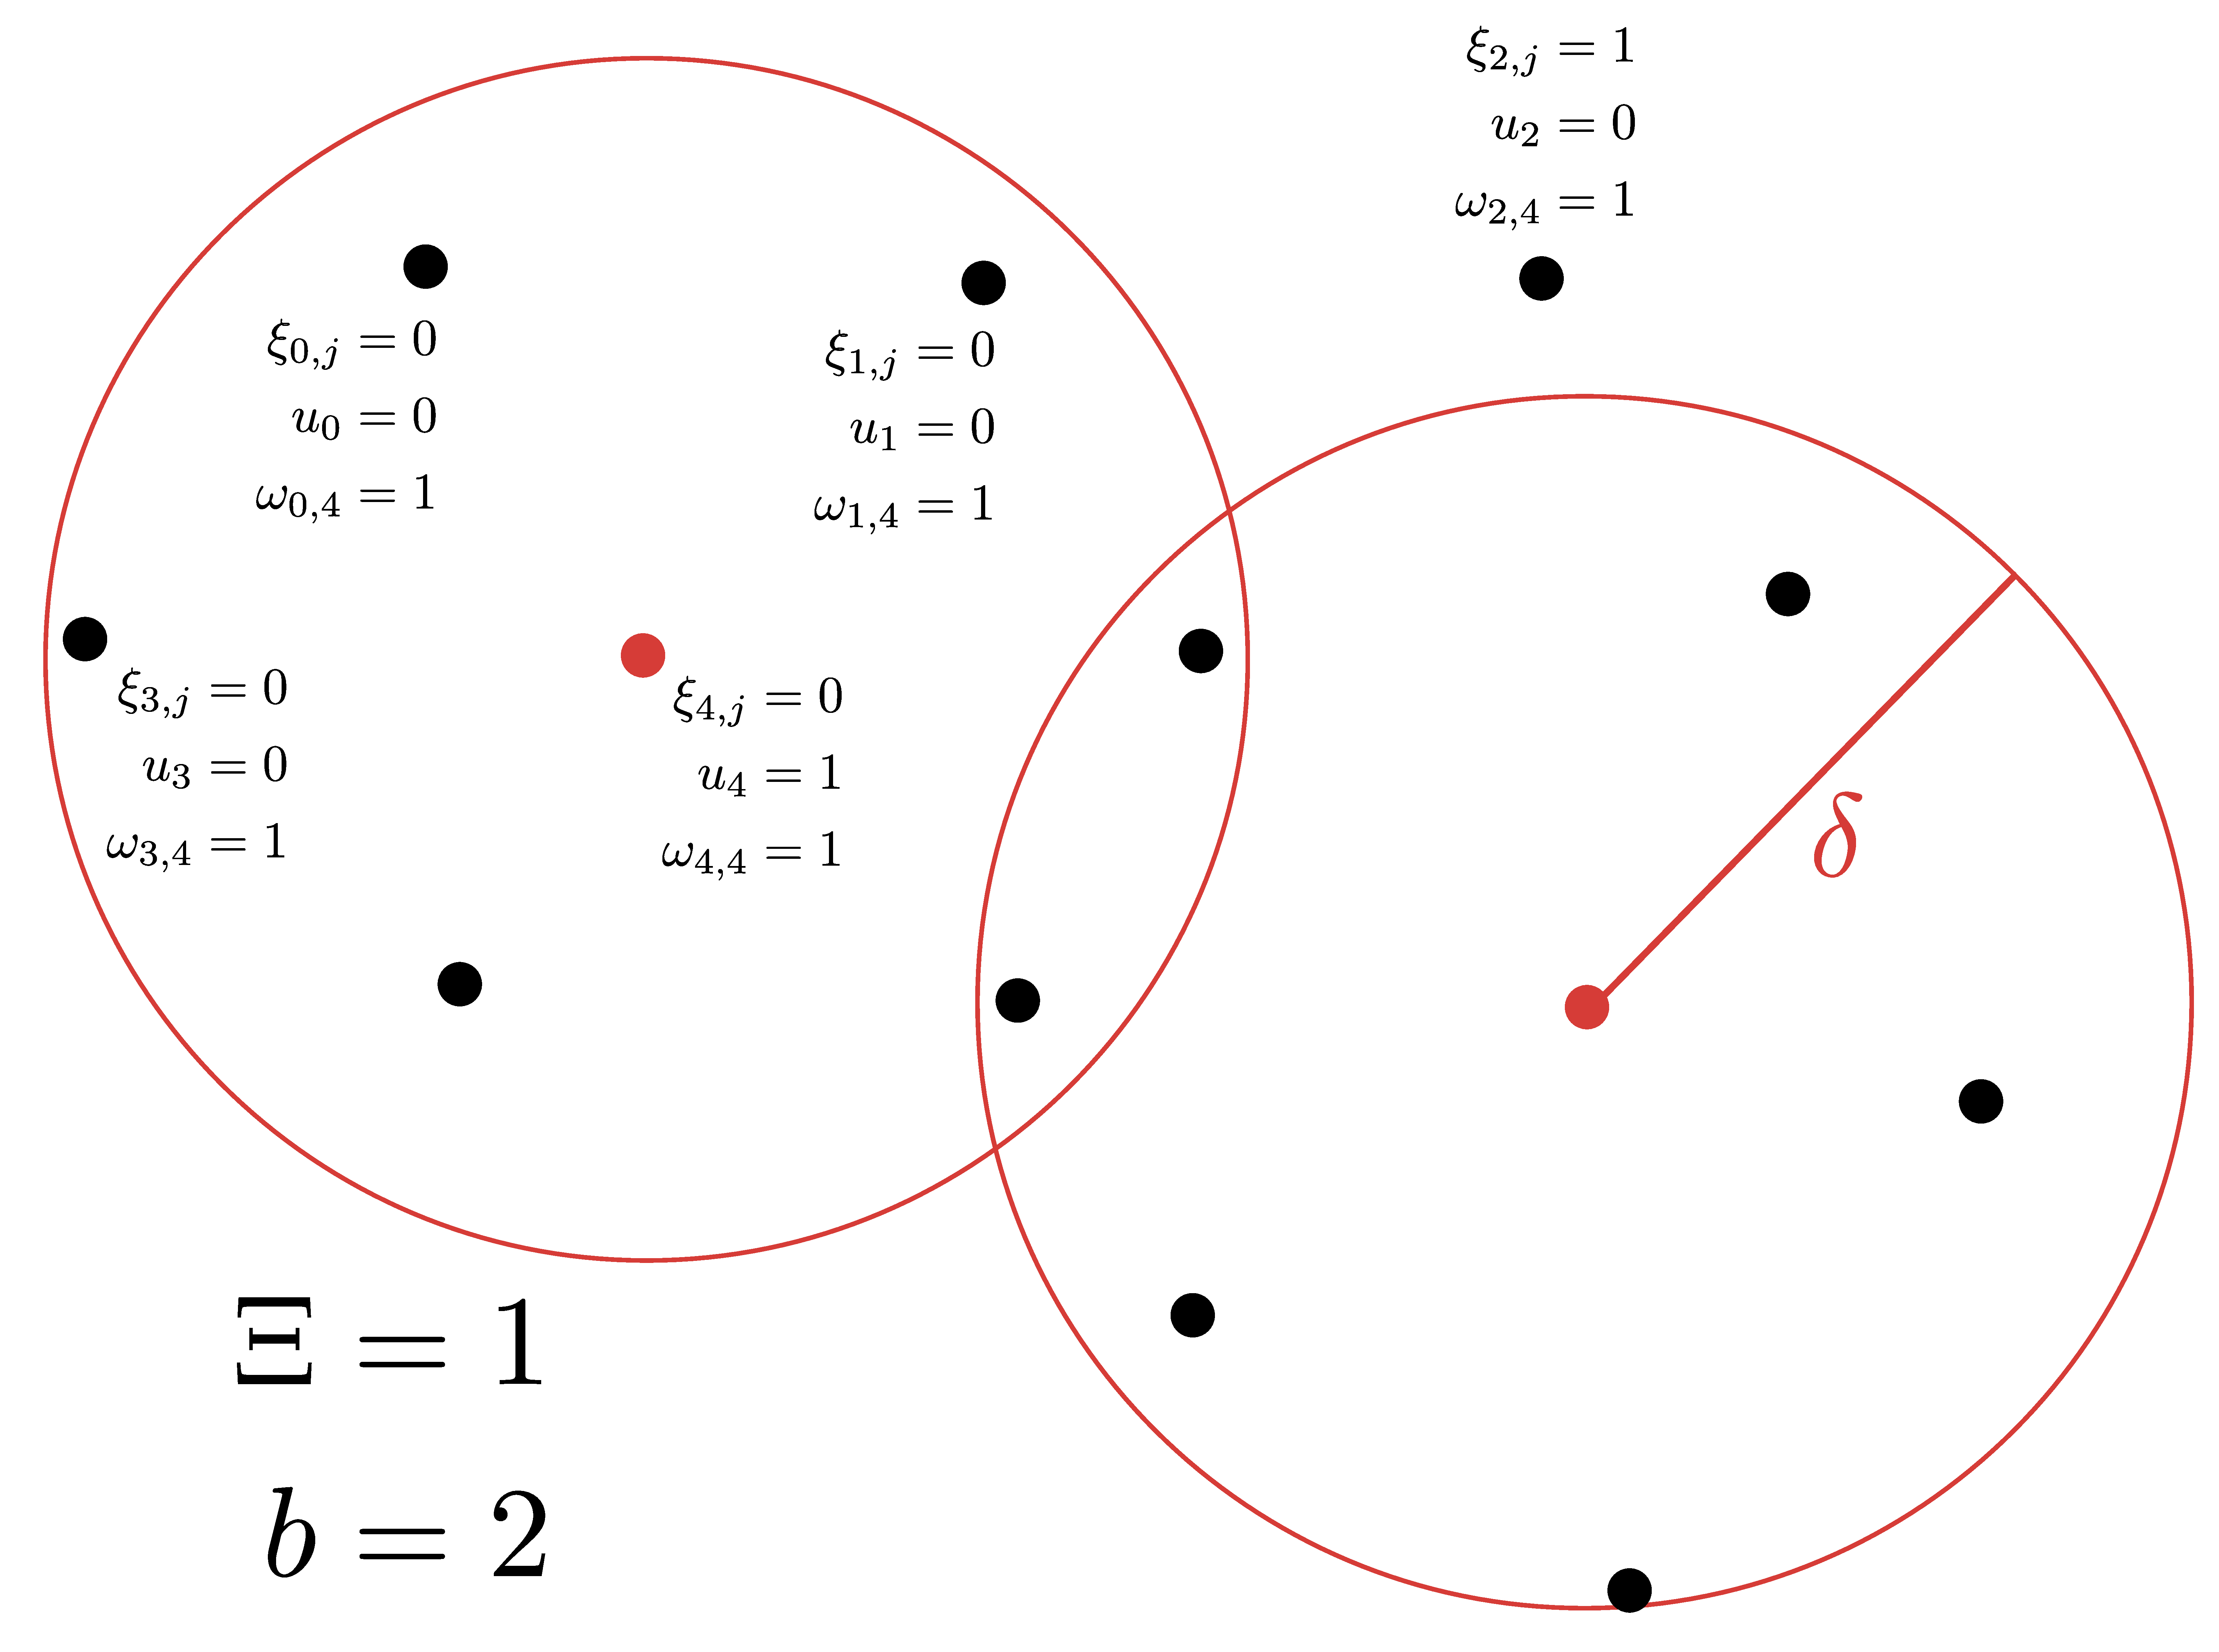
\includegraphics[width=0.38\textwidth]{mip.pdf}
\end{center}
    \caption{Visualizations of the variables in the mixed integer program. In this solution, the $4^{th}$ node is chosen as a center and node $0,1,3$ ended up in a $\delta$ ball around the $4^{th}$ node. The solution also marked the $2^{nd}$ node as an outlier by not including it in any $\delta$ ball.}
\label{mip}
\vspace{-12mm}
\end{wrapfigure}



\todo{Why retrain the model from scratch after collecting new labels (lines 764-765), rather than incrementally update the model?}

\subsection{Implementation Details}
\label{sec:imp}
One of the most important design choices is the distance function $\Delta(\cdot,\cdot)$. We use the $l_2$ distance between activations of the final fully-connected layer as a distance function. For semi-supervised learning, we used Ladder networks \cite{ladder} and for all experiments we used VGG-16 \cite{vgg} as the CNN architecture. We optimized all models using RMSProp with a learning rate of $1\mathrm{e}{-3}$ using Tensorflow \cite{tensorflow}. We train CNNs from scratch after each iteration of active learning step.

While implementing our algorithm, we used Gurobi \cite{gurobi} framework for checking feasibility of the MIP defined in (\ref{mipfeasible}). As an upper bound on number of outliers, we used $\Xi=1\mathrm{e}{-4} \times n$ where $n$ is the number of unlabelled data points.

%Upon acceptance, we are planning to release the trained models and the source code.
\section{Analysis of the Algorithm}
\label{sec:analysis}
In this section, we analyze our algorithm in terms of generalization error.  We are typically interested in the error in unseen images $E_{\mathbf{x},y \sim p_\mathcal{Z}}[l(\mathbf{x},y,A_{\mathbf{s}})]$ in terms of the empirical loss over the labelled images $\frac{1}{m}\sum_{j\in[m]} l(\mathbf{x}_{s(i)},y_{s(i)},A_{\mathbf{s}})$. However, this analysis requires joint treatment of the generalization error and the effect of query selection. For simplicity, we divide this analysis into two parts. First, we analyze the relationship between expected loss in unseen images (generalization error) and the empirical loss over the entire dataset ($\frac{1}{n}\sum_{i\in [n]} l(\mathbf{x}_i,y_i,A_\mathbf{s})$). Secondly, we analyze the relationship between the loss over the entire dataset and loss over the labelled samples. We study the first relationship by assuming a Lipschitz continuous loss function. By extending the robustness results from \cite{robust}, we state the following theorem and defer its proof to the supplementary material.

\begin{theorem}
Given $n$ i.i.d. samples drawn from $p_\mathcal{Z}$ as $\{\mathbf{x}_i,y_i\}_{i\in[n]}$. If loss function $l(\cdot,y,\mathbf{w})$ is $\lambda^l$-Lipschitz continuous for all $y, \mathbf{w}$, bounded by $L$ and $\mathcal{X}x\mathcal{Y}$ has a covering number $N_{\epsilon}(\mathcal{X},|\cdot|_2)=K$; with probability at least $(1-\delta)$,
\[
\left|E_{\mathbf{x},y \sim p_\mathcal{Z}}[l(\mathbf{x},y, A_\mathbf{s})] - \frac{1}{n}\sum_{i\in[n]} l(\mathbf{x}_i,y_i,A_\mathbf{s})\right|  \leq  \lambda^l \epsilon + L \sqrt{\frac{2K\log 2 + 2\log (1/\delta)}{n}}
\]
\label{mainthm}
\end{theorem}

First of all, this theorem is applicable to any machine learning algorithm with Lipschitz loss function and we further prove the Lipschitz-continuity of CNNs. It can clearly be seen that the empirical loss converges to the expected loss with large number of data points $n$ since $\lambda^l\epsilon$ term can be made arbitrarily small. In order to complete the study about the generalization performance of CNNs, we prove the Lipschitz-continuity of the loss function of a CNN with the following lemma where max-pool and restricted linear units are the non-linearities and the loss is defined as $l_2$ distance between the desired probabilities and the soft-max outputs.

\begin{lemma}
A convolutional neural network with $n_c$ convolutional (with max-pool and ReLU) and $n_{fc}$ fully connected layers defined over C class with loss function defined as 2-norm between softmax output and class probability is $\left(\frac{\sqrt{C-1}}{C} \alpha^{n_c+n_{fc}}\right)$-Lipschitz.
\end{lemma}

Here, $\alpha$ is the maximum sum of  input weights per neuron (see supplementary materials for formal definition). Although, it is in general unbounded, it can be made arbitrarily small without changing the loss function behavior (\ie keeping the label of any data point $\mathbf{s}$ unchanged). % since dividing all weights with a scalar will not switch any label. Hence, for any CNN, there is an equivalent CNN (in terms of classification function) with $\alpha \leq \varrho$ for any $\varrho > 0$. 
We can conclude that CNNs enjoy a $0$ generalization error in the limiting case thanks to the Lipschitz property.

In order to complete the analysis, we need to study the behavior of the loss over the dataset in terms of the empirical loss over the selected (queried) samples. Here, we make a no training error assumption; in other words, we assume that the training error for labelled images is $0$ at the end of the learning. This is clearly a restrictive assumption, however, it is very feasible due to large parameter space of CNNs. Moreover, this can also be enforced by simply converting average loss into maximal loss via \cite{maximal_loss}. %We did not need this trick since our CNNs reached 0 training error in all experiments. 
Using this assumption, we show that the loss over the entire dataset can be bounded using the result of our discrete optimization problem.% multiplied with a constant factor.

\begin{theorem}
Given $n$ i.i.d. samples drawn from $p_\mathcal{Z}$ as $\{\mathbf{x}_i,y_i\}_{i\in[n]}$, and $m$ chosen points $\{ s(i) \in [N]\}_{\i \in [m]}$. If loss function $l(\cdot,y,\mathbf{w})$ is $\lambda^l$-Lipschitz continuous for all $y, \mathbf{w}$ and bounded by $L$, regression function is $\lambda^\eta$-Lipschitz, $\{ s(i) \in [N]\}_{\i \in [m]}$ is $\delta$ cover of $\{\mathbf{x}_i,y_i\}_{i\in[n]}$, and $l(\mathbf{x}_{s(j)},y_{s(j)},A_\mathbf{S})=0\quad \forall j \in [m]$; with probability at least $1-\gamma$,
\begin{small}
\[
%\frac{1}{n}\sum_i l(\mathbf{x}_i,y_i,A_\mathbf{s}) \leq \mathcal{L}_{[n]} (h^\star) +\delta(\lambda^l + 2 \lambda^{\eta}) + 
%\sqrt{\frac{\log(1/1-\gamma)}{2n}}
\frac{1}{n}\sum_{i \in [n]} l(\mathbf{x}_i,y_i) \leq \delta (\lambda^l + \lambda^\mu LC)+ 
\sqrt{\frac{L \log(1/\gamma)}{2n}}
\]
\end{small}
%where $\mathcal{L}_{[n]} (h^\star)$ is the loss of the Bayes-optimal classifier.
\label{mainthm2}
\end{theorem}

It can easily be shown that in this setting, $\lim_{n \rightarrow \infty} \frac{1}{n}\sum_i l(\mathbf{x}_i,y_i,A_\mathbf{s}) =    \delta (\lambda^l + \lambda^\mu LC)$. Clearly, $\delta$ decreases when $m$ increases; however, the rate is critical. To show that our algorithm have finite query, we need to show that $\delta$ can be made arbitrarily small with finite $m$ in the limiting behavior of number of unlabelled data points (i.e. $n \rightarrow \infty$). Since our data points are coming from a compact space, there exists a finite sub-cover to any union of open sets. Hence, the finite query property is a straightforward result of compactness. %We give the following corollary without proof;

\iffalse
\begin{cor}
Given $n$ i.i.d. samples drawn from $p_\mathcal{Z}$ as $\{\mathbf{x}_i,y_i\}_{i\in[n]}$, and a desired error rate $\rho$. If loss function $l(\cdot,y,\mathbf{w})$ is $\lambda^l$-Lipschitz continuous for all $y, \mathbf{w}$, regression function is $\lambda^\eta$-Lipschitz, there exist a finite subset $\mathbf{s}$ with cardinality m such that any CNN achieving $0$ error over $\{\mathbf{x}_{s(j)},y_{s(j)}\}_{j \in [m]}$ achieve the following with probability $1$.
\[
\lim_{n \rightarrow \infty} \frac{1}{n}\sum_i l(\mathbf{x}_i,y_i) \leq \rho %\mathcal{L}_{[n]} (h^\star) +
\]
%where $\mathcal{L}_{[n]} (h^\star)$ is the loss of the Bayes-optimal classifier.
\label{maincor}
\end{cor}
\fi

In summary, we show that CNNs have Lipschitz continuous loss functions, making them generalize to unseen images. In addition, when the underlying data distribution has Lipschitz continuous regression functions, we further show, under reasonable assumptions, a small subset of dataset is enough to be labelled as long as it covers the space efficiently. Since the difference between the empirical loss over unseen images and the optimal loss is bounded by $\delta(\lambda^l + 2 \lambda^{\eta})$, direct minimization of $\delta$ is a theoretically soundapproach to this problem, validating our space-covering heuristic.


\begin{figure}[ht]
    \centering
    \begin{subfigure}[b]{\textwidth}
        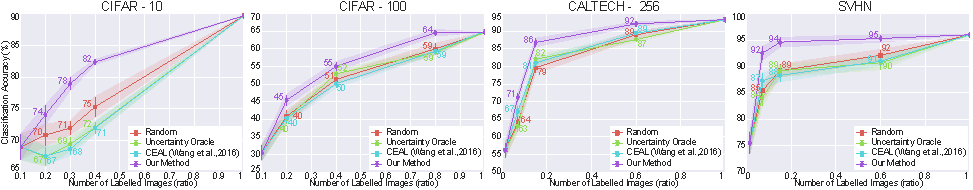
\includegraphics[width=\textwidth]{ws_fig2.pdf}
    \end{subfigure}
    \vspace{-5mm}
    \caption{Results on Active Learning for Weakly-Supervised Classifier}\label{fig:resnosemi}
        \vspace{-3mm}
    \label{fig:resns}
%\end{figure*}
%\begin{figure*}[ht]
%    \centering
   \vspace{5mm}
    \begin{subfigure}[b]{\textwidth}
        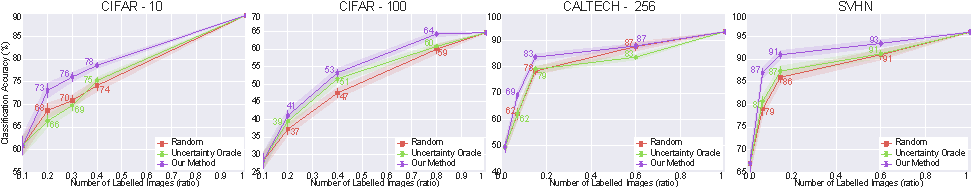
\includegraphics[width=\textwidth]{fs_fig2.pdf}
    \end{subfigure}
        \vspace{-5mm}
    \caption{Results on Active Learning for Fully-Supervised Classifier}\label{fig:ressemi}
        \vspace{-5mm}
    \label{fig:ress}
\end{figure}

\section{Experimental Results}
\label{sec:exp}

In order to evaluate our approach, we tested our algorithm on the problem of image classification. We used the CIFAR\cite{cifar} dataset in our experiments.  CIFAR\cite{cifar} dataset is composed of 50k images and each image is labelled with two different labels; one coarse-grained and one fine-grained. There are 100 fine-grained categories and 10 coarse-grained categories defined as strict super-sets of some of these fine-grained categories. 

We also performed experiments with and without semi-supervision. In our experiments, we start with 5k images sampled uniformly at random from the dataset as an initial pool. Semi-supervised algorithm has an access to labelled examples with their labels as well as unlabelled examples without their labels. Algorithms without semi-supervision have only access to the labelled data points. We use ladder networks\cite{ladder} for semi-supervision and the VGG16\cite{vgg} as a base architecture. We use the classification accuracy as a metric and plot the accuracy vs number of labelled points. At each step, we learned a network from scratch using $\mathbf{s}^{k} \cup \mathbf{s}^{k+1}$. We run the query algorithm iteratively; in other words, we solve the discrete optimization problem $\min_{\mathbf{s}^{k+1} : |\mathbf{s}^{k+1}| \leq b} E_{\mathbf{x},y \sim p_\mathcal{Z}} [l(\mathbf{x},y; A_{\mathbf{s}^{0} \cup \ldots, \mathbf{s}^{k+1}})]$ for each point on the accuracy vs number of labelled examples graph. We present the results in Figure~\ref{fig:ressemi}\&\ref{fig:resnosemi}.

We compare our algorithm with uniformly random sampling as well as the uncertainty oracle explained in Section~\ref{sec:whatif}. We also compared our algorithm with CEAL \cite{wang2016cost} which is to the best-of-our-knowledge, only active learning algorithm presented for CNNs. Since it is a semi-supervised approach utilizing unlabelled data points, we only include it in semi-supervised analysis.

 \begin{wrapfigure}{r}{0.5\textwidth}
\includegraphics[width=0.48\textwidth]{mip_100_2.pdf}
\caption{We compare our method with its greedy (k-CenterGreedy) version. Our algorithm provides both robustness and optimality with an additional computation cost and causes a small but not negligible accuracy improvement. }
\label{fig:twoopt}
\end{wrapfigure}

Figure~\ref{fig:resns} and \ref{fig:ress} suggests that our algorithm outperforms all other baselines; for the case of semi-supervised learning, with a large margin. We believe the effectiveness of our approach in semi-supervised case is because of the feature learning. In semi-supervised case, the feature learning is extremely important and having biased view of the space of images, will cause in inaccurate features. Since semi-supervision and active learning are two of the most promising directions in easing the cost of labelling for CNNs, we believe their joint analysis is extremely important. We also observed that our algorithm is less effective in CIFAR-100. We believe this is mostly due to the fact that there are $\sim500$ images per class in CIFAR-100 hence the effective dataset size per class is very small. Also, our theoretical analysis suggests our bound scales linearly with number of classes hence it is better have small number of classes.

\todo{All experiments are performed for 5 random initial labelled set selection, and we plot the average accuracy in the paper.  and error bars are 3-std-dev}

\todo{ CEAL is an active learning algorithm with weak supervision as it uses unlabelled images while training the classifier. Hence, improvement of CEAL is a results of their proposed weak supervision mechanism, rather than querying labels. Talk about caltech-256.}

\noindent\textbf{Optimality of the k-Center Solution:} Our proposed method is using the greedy 2-OPT solution for k-Center problem as an initialization and checks the feasibility of a mixed integer programming (MIP) program. Internally, we use LP-relaxation of the defined MIP and use branch-and-bound on the solution of the relaxed LP. Clearly, MIP does not enjoy a polynomial time solution; hence, the utility obtained by solving this expensive MIP should be investigated. We compare the average run-time of MIP\footnote{On Intel Core i7-5930K@3.50GHz and 64GB memory} with the run-time of 2-OPT solution in Table~\ref{tab:runtime}. We also compare the accuracy obtained with optimal k-Center solution and the 2-OPT solution in Figure~\ref{fig:twoopt}



\begin{table}[ht]
\centering
\vspace{-3mm}
\caption{Decomposition of average run-time of our discrete optimization algorithm for $b=5000$ and $|\mathbf{s}^0|=10000$ in seconds.}
\begin{tabular}{ccccc} \toprule
 Distance& Greedy & MIP & MIP &  \\
Matrix &(2-OPT) & (per iteration) & (total) & Total \\ \midrule
104.2  & 2   & 7.5  &  244.03  & 360.23  \\ \bottomrule
\end{tabular}
\label{tab:runtime}
\vspace{-2mm}
\end{table}

As shown in the Table~\ref{tab:runtime}; although the run-time of MIP is not polynomial in worst-case, in practice it converges in a tractable amount of time for a dataset of 50k images. %It should also be noted that the run time of our algorithm is negligible when compared with query time (asking oracle for labels). 
Hence, our algorithm can easily be applied in practice. %There are also many approximate and/or distributed solvers for both k-Center and MIP \cite{kcenterdist,gurobi}. %Hence, it can also scale to very large datasets of multiple million images.
 
Figure~\ref{fig:twoopt} suggests a small but significant drop on the accuracy when 2-OPT solution is used. Hence, we conclude that unless the scale of the dataset restricts, using our proposed optimal solver is desired. %It should also be noted that, we are not only solving k-Center problem optimally, we are also introducing robustness via slacked variables($\xi_{i,j}$). 
Even with the accuracy drop, our active learning strategy using 2-OPT solution still outperforms the other baselines. Hence, we can conclude that our algorithm can scale to any dataset size with small accuracy drop even if solving MIP is not possible.

\section{Conclusion}
We described an active learning algorithm for CNNs. Our empirical analysis showed that classical uncertainty based methods have limited applicability to the CNNs. We design a simple but effective active learning algorithm for CNNs using geometric intuitions. We further validated our algorithm using both theoretical analysis and an empirical study. Empirical results on CIFAR\cite{cifar} dataset showed state-of-the-art performance with a large-margin specifically for the semi-supervised case.


%{\small
\bibliography{active_adversarial} 
\bibliographystyle{abbrv}
%}

\appendix

\section{Proof for Lemma 1}
\begin{proof}
We will start with showing that softmax function defined over $C$ class is $\frac{\sqrt{C-1}}{C}$-Lipschitz continuous. It is easy to show that for any differentiable function \mbox{$f:\mathbb{R}^n\rightarrow\mathbb{R}^m$},

\[
\left \| f(\mathbf{x})-f(\mathbf{y})\right \|_2 \leq \left \|J\right \|^*_F  \left\| \mathbf{x}-\mathbf{y}\right\|_2  \, \, \forall \mathbf{x},\mathbf{y}\in\mathbb{R}^n
\]
where $\left \|J\right \|^*_F = \max\limits_{\mathbf{x}} \left \|J\right \|_F$ and $J$ is the Jacobian matrix of $f$.

Softmax function is defined as
\[
f(x)_i = \frac{\exp(x_i)}{\sum\limits_{j=1}^{C}\exp(x_j)}, \, i={1,2,...C}
\]
For brevity, we will denote $f_i(x)$ as $f_i$. The Jacobian matrix will be,
\[
J = \begin{bmatrix} f_1(1-f_1) & -f_1f_2  & ... & -f_1f_C \\
-f_2f_1 & f_2(1-f_2)  & ...  & -f_2f_C \\
... & ... & ... & ...  \\
-f_{C}f_{1} & -f_{C}f_{2}  & ...  & -f_{C}(1-f_{C})
\end{bmatrix}
\]
Now, Frobenius norm of above matrix will be,
\[
\left \| J \right \|_F = \sqrt{\sum\limits_{i=1}^{C}\sum\limits_{j=1 \\ i\neq j}^{C}f_{i}^{2}f_{j}^{2} + \sum\limits_{i=1}^{C} f_i^2(1-f_i)^2}
\]
It is straightforward to show that $f_i = \frac{1}{C}$ is the optimal solution for $\left \| J \right \|^{*}_F = \max\limits_{x}\left \| J \right \|_F $ Hence, putting $f_i = \frac{1}{C}$ in above equation , we get \mbox{$\left \| J \right \|^{*}_F = \frac{\sqrt{C-1}}{C}$}.

Now, consider two inputs $\mathbf{x}$ and $\mathbf{\tilde{x}}$, such that their representation at layer $d$ is $\mathbf{x}^d$ and $\mathbf{\tilde{x}}^d$. Let's consider any convolution or fully-connected layer as $\mathbf{x}^d_j = \sum_i w_{i,j}^d \mathbf{x}^{d-1}_i$. If we assume, \mbox{$\sum_i |w_{i,j}| \leq \alpha \quad \forall i,j,d$}.  For any convolutional or fully connected layer, we can state:
\[
\|\mathbf{x}^d - \mathbf{\tilde{x}}^d\|_2 \leq  \alpha \|\mathbf{x}^{d-1} - \mathbf{\tilde{x}}^{d-1}\|_2
\] 
On the other hand, using $|a-b| \leq |\max(0, a) - \max(0,a)|$ and the fact that max pool layer can be written as a convolutional layer such that only one weight is 1 and others are 0. We can further state that for ReLU and max-pool layers,
\[
\|\mathbf{x}^d - \mathbf{\tilde{x}}^d\|_2 \leq  \|\mathbf{x}^{d-1} - \mathbf{\tilde{x}}^{d-1}\|_2
\] 

Combining with the Lipschitz constant of soft-max layer,
\[
\|CNN(\mathbf{x};\mathbf{w}) - CNN(\mathbf{\tilde{x}};\mathbf{w})\|_2 \leq   \frac{\sqrt{C-1}}{C} \alpha^{n_c+n_{fc}}  \|\mathbf{x}-\mathbf{\tilde{x}}\|_2
\]
Since the loss function is $l_2$ as well, this concludes the proof.
\end{proof}

\section{Proof for Theorem 1}
In order to prove the Theorem 1, we extend the robustness bound from \cite{robust}.
\begin{proof}
\begin{small}
We will start with
\[
\begin{aligned}
&\left|E_{\mathbf{x},y \sim p_\mathcal{Z}}[l(\mathbf{x},y, A_\mathbf{s})] - \frac{1}{n}\sum_{i \in [n]} l(\mathbf{x}_i,y_i,A_\mathbf{s})\right| \\
&\overset{(a)}{\leq} \left|\sum_{j \in [K]} E[l(\mathbf{x},y)| (\mathbf{x},y) \in C_j] \mu_{j} -  \sum_{j \in [K]} E[l(\mathbf{x},y)| (\mathbf{x},y) \in C_j] \frac{|n_j|}{n} \right| \\
 &+  \left| \sum_{j \in [K]} E[l(\mathbf{x},y)| (\mathbf{x},y) \in C_j] \frac{|n_j|}{n}  - \frac{1}{n}\sum_{i \in [n]} l(\mathbf{x}_i,y_i) \right| \\
  &\overset{(b)}{\leq}\left|\sum_{j \in [K]} E[l(\mathbf{x},y)| (\mathbf{x},y) \in C_j] (\mu_{j} -   \frac{|n_j|}{n}) \right|
 +\frac{1}{n} \left|\sum_{j \in [K]} \sum_{i \in n_j} E[l(\mathbf{x},y)| (\mathbf{x},y) \in C_j]  - l(\mathbf{x}_i,y_i)\right| \\
   &\overset{(c)}{\leq} \left|\sum_{j \in [K]} E[l(\mathbf{x},y)|z \in C_j] (\mu_{j} -   \frac{|n_j|}{n})\right| + \lambda^l \epsilon  \\
 \end{aligned}
\]
\end{small}

Here, with brevity we denoted $l(\mathbf{x},y, A_\mathbf{s})$ as $l(\mathbf{x},y)$. In $(a)$, we used the fact that the space has an $\epsilon$ cover; and denote the cover as $\{C_j\}_{j \in [K]}$ such that each $C_j$ has diameter at most $\epsilon$. We further defined an auxiliary variable $\mu_j=p((\mathbf{x},y) \in C_j)$ and $n_j = \sum_i \mathds{1}[(\mathbf{x}_i,y_i) \in C_j]$ and used triangle inequality. In $(b)$, we used $i \in n_j$ to represent $(\mathbf{x}_i,y_i) \in C_j$. Finally, in $(c)$ we used the fact that each ball has diameter at most $\epsilon$ and the loss function is $\lambda^l$-Lipschitz. 
%Now, we will use the zero-loss of the classifier with Lipschitz continuity as;
%\[
%\begin{aligned}
%\left|\frac{1}{n}\sum_i l(A_s,x_i) \right| &= \left|\frac{1}{n}\sum_{j \notin {s(i)}_{i\in [M]}} l(A_s,x_i)  \right| \\
%&\leq  \frac{1}{n}\sum_{j \notin {s(i)}_{i\in [M]}} \lambda  \left| \mathbf{x}_i - \mathbf{x}_k\right | \leq \frac{n-m}{n} \lambda \tilde{\epsilon}
%\end{aligned}
%\]
%Combining both,
%\[
%\begin{aligned}
%&E[l(A_s,z)] \leq  \left|E[l(A_s,z)] - \frac{1}{n}\sum_i l(A_s,x_i) \right|  \\ &+ \left|\frac{1}{n}\sum_i l(A_s,x_i) - \frac{1}{m}\sum_i l(A_s,x_{s(i)}) \right| \\
%&\leq \left|\sum_{j} E[l(A_s,z)|z \in C_j] (\mu_{j} -   \frac{|N_j|}{n})\right| +\epsilon(s) + \frac{n-m}{n} \lambda \tilde{\epsilon}
%\end{aligned}
%\]

We can bound $E[l(\mathbf{x},y)|z \in C_j]$ with maximum loss $L$ and use Breteganolle-Huber-Carol inequality (\emph{cf} Proposition A6.6 of \cite{wellner}) in order to bound $\sum_{j} \mu_{j} -   \frac{|n_j|}{n}$. 

Combining all; with probability at least $(1-\delta)$,
\[
\left|E_{\mathbf{x},y \sim p_\mathcal{Z}}[l(\mathbf{x},y, A_\mathbf{s})] - \frac{1}{n}\sum_{i \in [n]} l(\mathbf{x}_i,y_i,A_\mathbf{s})\right| \leq  \lambda^l \epsilon + L \sqrt{\frac{2K\log 2 + 2\log (1/\delta)}{n}}
\]
\end{proof}

\section{Proof for Theorem 2}
Before starting our proof, we state the Claim 1 from \cite{BerlindU15}. Fix some $p,p^\prime \in [0,1]$ and $y^\prime \in \{0,1\}$. Then,
\[
p_{y \sim p}(y \neq y^\prime) \leq p_{y \sim p^\prime}(y \neq y^\prime) + |p - p^\prime|
\]
\begin{proof}
We will start our proof with bounding $E[l(\mathbf{x}_i,y_i)]$. We have a condition which states that there exists and $\mathbf{x}_j$ in $\delta$ ball around $\mathbf{x}_i$ such that $\mathbf{x}_j$ has $0$ loss.
\[
\begin{aligned}
E[l(\mathbf{x}_i,y_i)] &= \sum_{k\in [C]} p_{y_i \sim \eta_k(\mathbf{x}_i)}(y_i = k) l(\mathbf{x}_i,k) \\
&\overset{(d)}{\leq} \sum_{k\in [C]} p_{y_i \sim \eta_k(\mathbf{x}_j)}(y_i = k) l(\mathbf{x}_i,k) \\ &\quad+ \sum_{k\in [C]}  |\eta_k(\mathbf{x}_i)-\eta_k(\mathbf{x}_j)| l(\mathbf{x}_i,k) \\
&\overset{(e)}{\leq} \sum_{k\in [C]} p_{y_i \sim \eta_k(\mathbf{x}_j)} (y_i = k) l(\mathbf{x}_i,k) + \delta \lambda^\eta L C\\ 
\end{aligned}
\]
With abuse of notation, we represent \mbox{$\{y_i=k\} \sim \eta_k(\mathbf{x}_i)$} with \mbox{$y_i \sim \eta_k(\mathbf{x}_i)$}. We use Claim 1 in $(d)$, and Lipschitz property of regression function and bound of loss in $(d)$. Then, we can further bound the remaining term as; 
\[
\begin{aligned}
&\sum_{k\in [C]} p_{y_i \sim \eta_k(\mathbf{x}_j)} (y_i = k) l(\mathbf{x}_i,k) \\
&= \sum_{k\in [C]} p_{y_i \sim \eta_k(\mathbf{x}_j)} (y_i = k) [l(\mathbf{x}_i,k) - l(\mathbf{x}_j,k) ] \\ &\quad+ \sum_{k\in [C]} p_{y_i \sim \eta_k(\mathbf{x}_j)} (y_i = k) l(\mathbf{x}_j,k) \\
&\leq \delta \lambda^l
\end{aligned}
\]
where last step is coming from the fact that the trained classifier assumed to have $0$ loss over training points. If we combine them,
\[
E[l(\mathbf{x_i},y_i)] \leq \delta( \lambda^l+\lambda^\mu LC)
\]
We further use the Hoeffding's Bound and conclude that with probability at least $1 - \gamma$,
\[
\frac{1}{n}\sum_{i \in [n]} l(\mathbf{x}_i,y_i) \leq \delta (\lambda^l + \lambda^\mu LC)+ 
\sqrt{\frac{L \log(1/\gamma)}{2n}}
%\frac{\log(1/(1-\delta)){2n}
\]
\end{proof}

\section{Unsupervised subset selection} 

Since our algorithm does not use any uncertainty information, we can also use it for unsupervised subset selection. In other words, given an informative distance function, we can use our algorithm to choose subset of the training set. In unsupervised subset selection problem, the constraint is using subset of the dataset due to the resource constraints. Given a dataset size constraint, the problem is choosing a subset of examples such that the trained model will perform as closely as possible to the model trained on entire dataset. One big difference to active learning is lack of iteration. Given a budget, subset is selected and not refined/improved.


We perform this experiment with $l_2$ distance of features learned with no supervision as $\Delta(\cdot,\cdot)$. We use \cite{improved_gan} for unsupervised feature learning using their shared source code. We plot the accuracy vs dataset size using both our algorithm and uniformly random selection in Figure~\ref{fig:scat} and conclude that our algorithm is effective for the problem of unsupervised subset selection.  

\begin{wrapfigure}{r}{0.5\textwidth}
\includegraphics[width=0.5\textwidth]{u_100_2.pdf}
\caption{Experiment on unsupervised subset selection. We use our algorithm with ImprovedGAN\cite{improved_gan} features in unsupervised subset selection setup. Results suggest that our algorithm is more effective than uniform random sampling .}
\label{fig:scat}
\end{wrapfigure}

\end{document}
